\documentclass[10pt,a4paper]{article}
\usepackage[left=1.5cm,right=1.5cm,top=1.5cm,bottom=1.5cm]{geometry}
\usepackage[utf8]{inputenc}
\usepackage[english]{babel}
\usepackage{amsmath}
\usepackage{amsfonts}
\usepackage{amssymb}
\usepackage{graphicx}
\usepackage{listings}
\usepackage{enumitem}
\usepackage{wrapfig}


\setitemize{itemsep=0ex}
\renewcommand{\labelitemi}{--}
\renewcommand{\labelitemii}{$\infty$}
\renewcommand{\arraystretch}{1.5}
\linespread{1}


\title{Distributed Systems\\Zusammenfassung}
\author{Frédéric Vogel}
\date{ETH Zürich, HS14}

\begin{document}
\maketitle

\tableofcontents

\pagebreak

\section{Teil 1}
\subsection{Definition und Historie}
\begin{quote}
A distributed computing system consists of multiple autonomous processors that do not share primary memory, but cooperate by sending messages over a communication network.

\textsc{H. Bal}
\end{quote}


\subsection{Architekturen verteilter Systeme}
\subsubsection{Peer-to-Peer (P2P)}
\begin{itemize}
\item Jeder Rechner gleichzeitig Informationsanbieter und -konsument
\end{itemize}

\subsubsection{Client-Server}
\begin{itemize}
\item Server als Informationsanbieter (reagierender Prozess)
\item Client als Konsument (initiierender Prozess)
\item Client gleichzeitig Benutzungsschnittstelle
\item WWW-dominiertes Internet
\end{itemize}

\subsubsection{3-Tier}
\begin{itemize}
\item Verarbeitung wird auf mehrere physikalische Einheiten verteilt
\item Logische Schichten mit minimierten Abhängigkeiten
\item Leichtere Wartung, einfaches Austauschen
\end{itemize}

\subsubsection{Multi-Tier}
\begin{itemize}
\item Weitere Schichten, mehrere physikalische Einheiten pro Schicht $\rightarrow$ erhöht Skalierbarkeit und Flexibilität
\item Mehrere Server ermöglichen Lastverteilung
\item Verteilte Datenbanken bietet Sicherheit (Replikation, hoher Durchsatz)
\end{itemize}

\subsubsection{Compute-Cluster}
\begin{itemize}
\item Vernetzung kompletter Einzelrechner
\item Räumlich konzentriert (wenige Meter)
\item Sehr schnelles Verbindungsnetz
\item Diverse Netztopologien, sehr unterschiedlich hinsichtlich
\begin{itemize}
\item Skalierbarktei
\item Routingkomplexität
\item usw.
\end{itemize}
\end{itemize}

\subsubsection{Service-Oriented Architecture (SOA)}
\begin{itemize}
\item Unterteilung der Applikation in einzelne, unabhängige Abläufe innerhalb eines Geschäftsprozess $\rightarrow$ erhöht Flexibilität
\item Lose Koppelung zwischen Services über Nachrichten und Events
\item "Development by composition": Services können bei Änderungen der Prozesse einfach neu zusammengestellt werden
\item Services können von externen Anbietern bezogen werden
\item Oft in Zusammenhang mit Web-Services
\end{itemize}

\subsubsection{Cloud-Computing}
\begin{itemize}
\item Massive Bündelung der Rechenleistung an zentraler Stelle
\item Outsourcen von Applikationen in die Cloud
\item Internet nur noch als Vermittlungsinstanz
\end{itemize}


\subsection{Charakteristika \& Phänomene}
\begin{itemize}
\item Neue Probleme durch räumliche Separation und Autonomie der Komponenten:
\begin{itemize}
\item partielles Fehlverhalten möglich (statt totaler Absturz)
\item fehlender globaler Zustand / exakt synchronisierte Zeit
\item mögliche Inkonsistenzen (z.B. zwischen Datei und Verzeichnis/Index)
\end{itemize}
\item Heterogenität in Hard- und Software
\item Hohe Komplexität
\item Sicherheit notwendiger aber schwieriger
\end{itemize}

\subsubsection{Beispiele konzeptioneller Probleme}
\begin{description}
\item[Schnappschussproblem] Wie viel Geld ist im Umlauf?
\begin{itemize}
\item Ständige Transfers
\item Keine globale Sicht
\item Keine gemeinsame Zeit
\end{itemize}
\item[Deadlock] Zyklische Wartebedingung
\item[Uhrensynchronisation] Uhren gehen nicht gleich schnell, keine globale Zeit
\item[Kausaltreue Beobachtungen] Gewünscht:  Ursache stets vor ihrer (u.U. indirekten) Wirkung beobachten
\item[Verteile Geheimnisvereinbarung] Einigung eines gemeinsames geheimes Passwort über unsicheren Kanälen
\end{description}


\subsection{Kommunikation --- Nachrichten}
Prozesse sollen kooperieren, daher untereinander Information austauschen können.
\begin{itemize}
\item Globaler Speicher (physisch oder virtuell)
\item Nachrichten
\end{itemize}

\subsubsection{Nachrichtenbasierte Kommunikation}
\begin{itemize}
\item Send $\rightarrow$ Receive
\item Implizierte Synchronisation, Senden vor Empfangen
\end{itemize}

\subsubsection{Ordungserhalt von Nachrichten}
\begin{description}
\item[FIFO] First In, First Out\\Empfangsreihenfolge = Sendereihenfolge (zwischen zwei Prozessen)
\item[Kausale Ordnung] Keine Information erreicht Empfänger auf Umwegen schneller als auf direktem Wege\\Globalisierung von FIFO auf mehrere Prozesse
\end{description}

\subsubsection{Fehlermodelle}
\begin{description}
\item[Nachrichtenfehler beim Senden/Übertragen/Empfangen]  \hfill \\Verlorene Nachricht
\item[Crash / Fail-Stop: Ausfall eines Prozessors] \hfill \\Nicht mehr erreichbarer/mitspielender Prozess
\item[Zeitfehler] \hfill \\Ereignis geschieht zu spät oder zu früh
\item[Byzantinische Fehler] \hfill \\Beliebiges Fehlverhalten, z.B.:
\begin{itemize}[topsep=-100ex]
\item Verfälschte Nachrichteninhalte
\item Prozess, der unsinnige Nachrichten sendet
\end{itemize}
\end{description}

\subsubsection{Mitteilungsorientierte Kommunikation}
\begin{itemize}
\item Einfachste Form der Kommunikation
\item Unidirektional
\end{itemize}

\subsubsection{Auftragsorientierte Kommunikation}
\begin{itemize}
\item Bidirektional
\item Ergebnis des Auftags wird als Antwortnachricht zurückgeschickt
\end{itemize}


\subsection{Kommunikation --- synchron/asynchron}
\begin{description}
\item[Blocking send] \hfill\\ Sender ist bis zum Abschluss der Nachrichtentransaktion blockiert\\Sender hat Garantie Nachricht wurde zugestell/empfangen
\item[Synchrone Kommunikation] \hfill\\ Send und receive geschehen (im Prinzip) gleichzeitig
\item[Virtuelle Gleichzeitigkeit] \hfill\\ Bei Abstraktion von Realzeit ist ein Ablauf durch ein äquivalentes Zeitdiagramm darstellbar, bei dem alle Nachrichtenpfeile senkrecht verlaufen\\Nur stetige Deformation erlaubt (verschieben auf Zeitachse, nicht kreuzen)
\item[Asynchrone Kommunikation / No-wait send] \hfill\\ Send und receive nicht gleichzeitig\\Sender nur bis zur lokalen Ablieferung der Nachricht an das Transportsystem blockiert
\end{description}

\subsubsection{Asynchrone $\leftrightarrow$ synchrone Kommunikation}
\paragraph{Vorteile asynchroner Kommunikation}
\begin{itemize}[topsep=-100ex]
\item sendender Prozess kann weiterarbeiten während Nachricht übertragen wird
\item stärkere Entkopplung von Sender und Empfänger
\item höherer Grad an Parallelität möglich
\item geringere Gefahr von Deadlocks
\end{itemize}
\paragraph{Nachteile}
\begin{itemize}[topsep=-100ex]
\item Sender weiss nicht, ob/wann Nachricht angekommen ist
\item Debugging der Anwendung oft schwierig
\item System muss Puffer verwalten
\end{itemize}

\subsubsection{Synchron $\stackrel{?}{=}$ blockierend}
\begin{description}
\item[Blockierung] Rein senderseitiger Aspekt
\begin{description}
\item[blockierend] Sender wartet, bis Nachricht lokal vom Kommunikationssystem abgenommen wurde
\item[nicht-blockierend]Sender informiert Kommunikationssystem, dass \& wo zu versendende Nachricht ist
\end{description}
\item[Synchron/asynchron] Nimmt Bezug auf Empfänger
\begin{description}
\item[synchron] Nach Ende der Send-Operation wurde Nachricht dem Emfpänger zugestellt
\item[asynchron] Nicht garantiert
\end{description}
\end{description}

\subsubsection{Hauptklassifikation von Kommunikationsmechanismen}
\begin{tabular}{l || l | l}
 & asynchron & synchron\\
 \hline \hline
 Mitteilung & no-wait send & Rendezvous\\
 \hline
 Auftrag & asynchroner RPC & Remote Procedure Call (RPC)
\end{tabular}
\linebreak\\
Häufigste Kombination: Mitteilung asynchron, Auftrag synchron

\paragraph{No-wait send}
\begin{itemize}
\item[$\oplus$]weitgehende zeitliche Entkopplung von Sender und Empfänger
\item[$\oplus$]einfache, effiziente Implementierung (bei kurzen Nachrichten)
\item[$\circleddash$]keine Erfolgsgarantie für Sender
\item[$\circleddash$]Notwendigkeit der Zeishcenpufferung
\item[$\circleddash$]Gefahr des "Überrennens" des Empfängers bei zu häufigen Nachrichten
\end{itemize}
\begin{figure}[h]
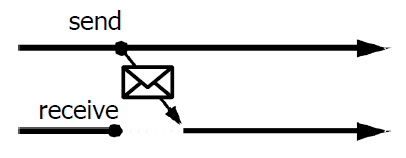
\includegraphics[scale=0.33]{./Bilder/No-wait_send}
\end{figure}

\paragraph{Rendezvous-Protokolle}
\begin{itemize}
\item Der erste wartet auf den anderen (Synchronisationspunkt)
\item Mit NACK/ACK wenig Puffer nötig aber aufwändiges Protokoll (busy waiting)
\end{itemize}
\begin{figure}[h]
\includegraphics[scale=0.33]{./Bilder/Rendezvous-Protokolle}
\end{figure}


\subsection{Kommunikation --- RPC}
\begin{itemize}
\item Aufruf einer entfernten Prozedur
\item Soll klassischem Prozeduraufruf möglich gleichen (klare Semantik für Anwender)
\item Einfaches Programmieren
\begin{itemize}
\item kein Erstellen von Nachricht, kein Quittieren, etc. auf Anwendungsebene
\item Syntax analog zu lokalem Prozeduraufruf
\item Typsicherheit (Datentypprüfung auf Client- und Serverseite möglich)
\end{itemize}
\end{itemize}
\begin{figure}[h]
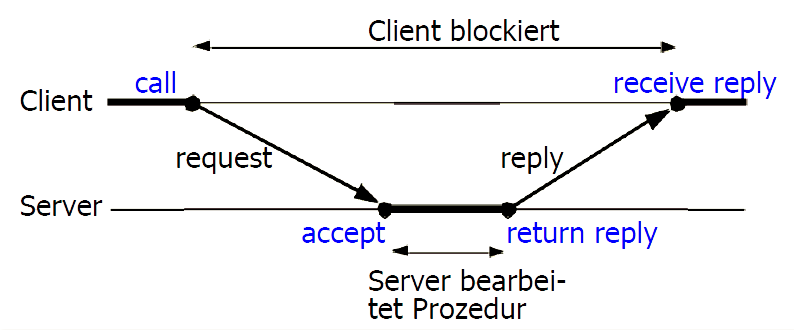
\includegraphics[scale=0.33]{./Bilder/RPC}
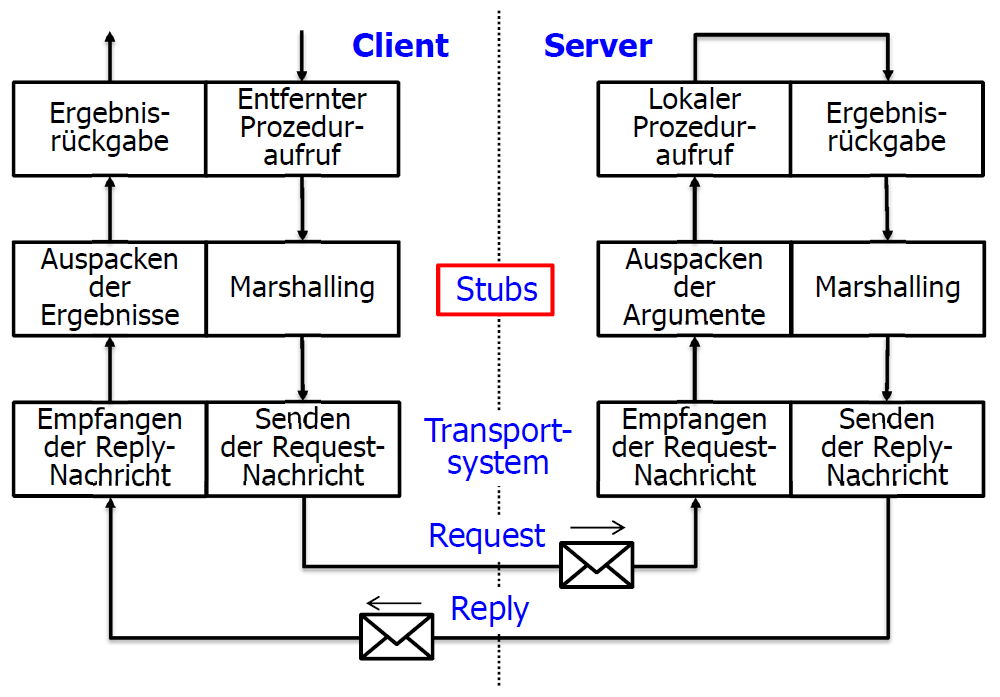
\includegraphics[scale=0.25]{./Bilder/RPC_Implementierung}
\end{figure}


\subsubsection{RPC: Stubs}
\paragraph{Client-Stub}
\begin{lstlisting}
call S.X(out: a; in: b);
\end{lstlisting}
wird ersetzt durch längeres Programmstück (Stub), welches:
\begin{itemize}
\setlength{\itemsep}{0cm}%
\setlength{\parskip}{0cm}%
\item Parameter a in Nachricht packt
\item Nachricht an Server S sendet
\item Timeout für Antwort setzt
\item Antwort entgegennimmt
\item Erreignisparameter b mit Werten der Antwortnachricht setzt 
\end{itemize}

Stubs
\begin{itemize}
\item wirken als proxy (lokale Stellvertreter des entfernten Gegenüber
\item simulieren einen lokalen Aufruf
\item sorgen für Zusammenbau und Entpacken von Nachrichten
\item konvertieren Datenrepräsentationen
\item können weitgehend automatisch generiert werden
\item steuern das Übertragungsprotokoll
\end{itemize}

\subsubsection{Probleme mit RPC}
Soll möglichst aussehen wie lokaler Prozeduraufruf, doch
\begin{itemize}
\item Server kann unerreichbar/abgestürtzt sein
\item RPCs dauern länger
\item Anwender hat keine Kontrolle über Server
\item Ungewisse, variable Verzögerungen
\item Keine Kommunikation über globale Variablen
\item Keine Pointer/Referenzparameter als Parameter möglich
\item mehr Fehlerfälle (Server-/Client-Absturz, Nachrichtenverlust, etc.)
\end{itemize}

\paragraph{Verlorene Request-Nachricht}
\begin{description}
\item[Gegenmassnahme]\hfill\\
Nach Timeout Request-Nachricht erneut senden
\item[Probleme]\hfill\\
\begin{itemize}[topsep=-100ex]
\item Wie viele Wiederholungsversuche maximal?
\item Wie gross soll Timeout sein?
\item Was wenn Nachricht nicht verloren sondern untypisch langsam?
\end{itemize}
\item[Probleme wenn Nachricht tatsächlich nicht verloren]\hfill\\
\begin{itemize}[topsep=-100ex]
\item Doppelte Request-Nachricht (gefährlich bei nicht-idempotente serverseitige Operation)
\item Server sollte solche Duplikate erkennen
\end{itemize}
\end{description}

\paragraph{Verlorene Reply-Nachricht}
\begin{description}
\item[Gegenmassnahme 1]\hfill\\
Analog zu verlorener Request-Nachricht
\item[Probleme]\hfill\\
\begin{itemize}[topsep=-100ex]
\item Vielleicht ging Request verloren?
\item Server war langsam und arbeitet noch?
\item Nicht unterscheidbar aus Client-Sicht
\end{itemize}
\item[Gegenmassnahme 2]\hfill\\
Server hält Historie versendeter Replies
\begin{itemize}[topsep=-100ex]
\item Falls Duplikat erkannt wird und Auftrag bereits ausgeführt: letztes Reply erneut senden
\item Pro Client nur letztes Reply speichern
\item Nach gewisser Zeit Historie löschen
\end{itemize}
\end{description}

\paragraph{Server-Crash}
\begin{description}
\item[Probleme]\hfill\\
\begin{itemize}[topsep=-100ex]
\item Wie soll Client untere Fälle unterscheiden?
\item Client meint evtl. zu Unrecht, dass Auftrag nicht ausgeführt wurde
\end{itemize}
\end{description}
\begin{figure}[h]
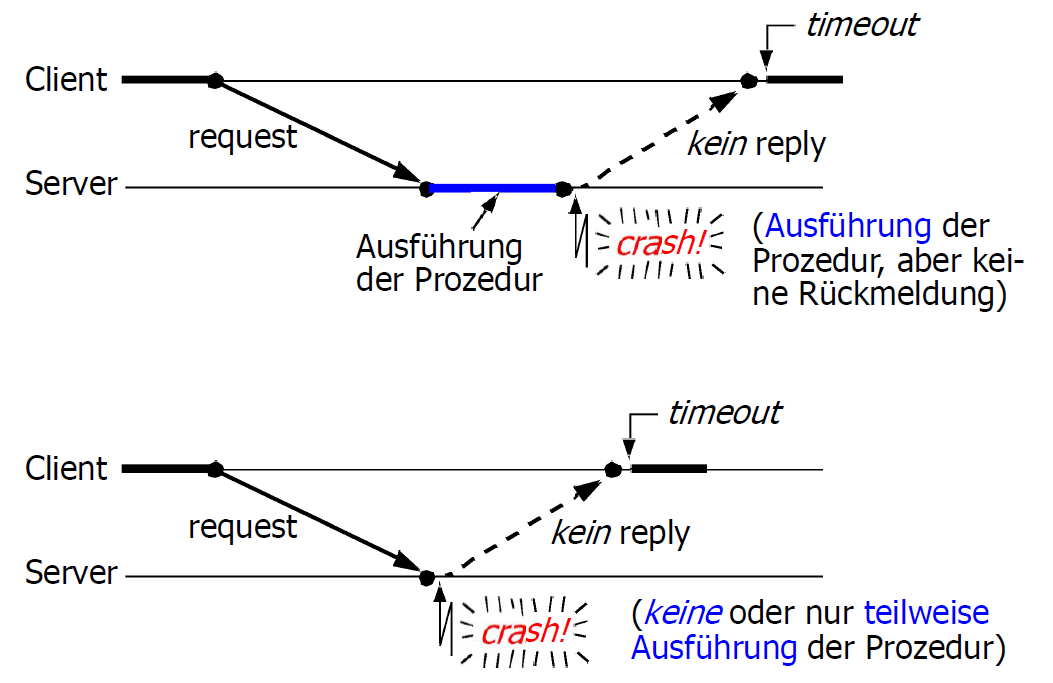
\includegraphics[scale=0.15]{./Bilder/Server-Crash}
\end{figure}

\paragraph{Client-Crash}
\begin{description}
\item[Probleme]\hfill\\
\begin{itemize}[topsep=-100ex]
\item Reply des Servers wird nicht abgenommen $\rightarrow$ blockiert Ressourcen bei Server
\item Orphans beim Server
\item Server fragt ab und zu ob Client noch an Antwort interessiert (bzw. ob Client existiert)
\end{itemize}
\end{description}
\begin{figure}[h]
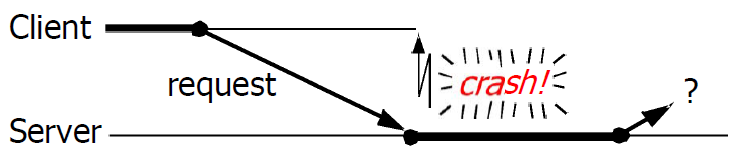
\includegraphics[scale=0.2]{./Bilder/Client-Crash}
\end{figure}

\subsubsection{RPC-Fehlersemantik-Klassen}
\paragraph{Maybe-Semantik}
\begin{itemize}
\item Keine Wiederholung von Requests
\item Einfach und effizient
\item Keinerlei Erfolgsgarantien $\rightarrow$ nur ausnahmsweise anwendbar
\item Mögliche Anwendungen: Auskunftsdienste
\end{itemize}

\paragraph{At-least-once-Semantik}
\begin{itemize}
\item Automatische Wiederholung von Requests
\item Keine Duplikatserkennung (zustandsloses Protokoll auf Serverseite)
\item Akzeptabel bei idempotenten Operationen (z.B. Lesen einer Datei)
\end{itemize}

\paragraph{At-most-once-Semantik}
\begin{itemize}
\item Erkennen von Duplikaten (Sequenznummern, log-Datei, etc.)
\item Keine wiederholte Ausführung der Prozedur
\item Geeignet auch für nicht-idempotente Operationen
\end{itemize}

\subsubsection{Asynchroner RPC}
\begin{itemize}
\item Auftragsorientiert $\rightarrow$ Antwortverpflichtung
\item Parallelverarbeitung von Client und Server möglich (solange Client nicht auf Resultat angewiesen)
\end{itemize}
\begin{figure}[h]
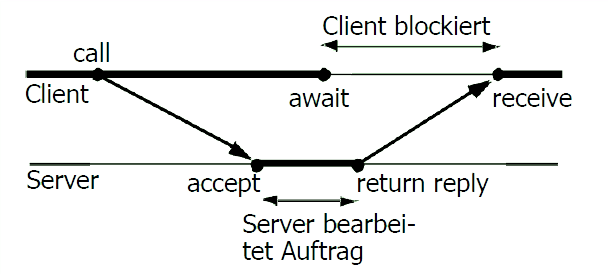
\includegraphics[scale=0.2]{./Bilder/Asynchroner_RPC}
\end{figure}


\subsection{Client/Server}
\begin{description}
\item[Client]\hfill\\Konsument, initiierender Prozess, Benutzungsschnittstelle
\item[Server]\hfill\\Informationsanbieter, reagierender Prozess
\end{description}

\subsubsection{Gleichzeitige Server-Aufträge}
Problem: Oft viele gleichzeitige Aufträge

\paragraph{Iterativer Server: }Bearbeitet nur einen einzigen Auftrag pro Zeit
\begin{itemize}
\item einfach zu realisieren
\item eintreffende Anfragen puffern, abweisen oder ignorieren
\item sinnvoll bei trivialen Diensten mit kurzer Bearbeitungszeit
\end{itemize}
\begin{figure}[h]
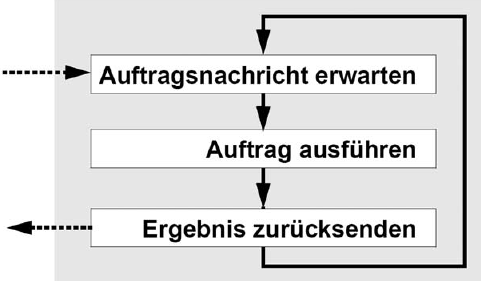
\includegraphics[scale=0.5]{./Bilder/Iterativer_Server}
\end{figure}

\paragraph{Konkurrent-Server: }Quasi-gleichzeitige Bearbeitung mehrerer Aufträge

Sinnvoll bei längeren Aufträgen

\paragraph{Konkurrente Server mit dynamischen Handler-Prozessen: }Master gründet Slave-Prozess für jeden Auftrag
\begin{itemize}
\item Neu gegründeter Slave übernimmt den Auftrag
\item Client kommuniziert direkt mit Slave
\item Slaves typischerweise Leichtgewichtprozesse
\item Slaves terminieren nach Auftrag
\item Anzahl gleichzeitiger Slaves begrenzt
\end{itemize}
\begin{figure}[h]
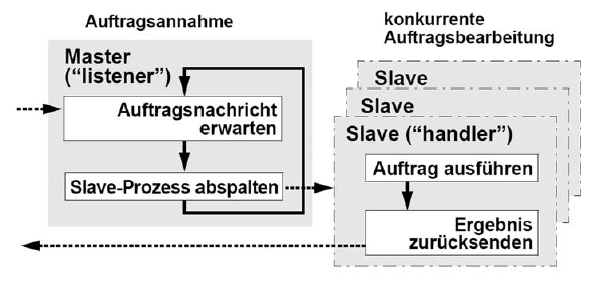
\includegraphics[scale=0.5]{./Bilder/Konkurrente_Server_dynamische_handler_prozesse}
\end{figure}

\subsubsection{Stateless/statefull Server}
\begin{itemize}
\item Hält Server Zustandsinformation über Aufträge hinweg?
\item Bei zustandslosen Servern muss jeder Auftrag vollständig beschrieben sein (Position Dateizeiger, etc.)
\item Dateisperren bei zustandslosen Servern nicht einfach möglich
\item Zustandsbehaftete Server im Allg. effizienter
\item Zustandsbehaftete Server können wiederholte Aufträge erkennen $\rightarrow$ Idempotenz
\item Crash eines Servers gibt weniger Probleme im zustandslosen Fall
\end{itemize}

\subsubsection{Wiedererkennung von Kunden}
\paragraph{URL Rewriting und dynamische Websites}
\begin{itemize}
\item der Einstiegsseite eindeutige Identität anheften wenn Kunde erstmals Seite aufruft
\item Identität jedem Link auf Seite anheften und mit übertragen
\item Gefahr: Identität klauen durch wissen der URL
\end{itemize}

\paragraph{Cookie als Context-Handle}
\begin{itemize}
\item Textdatei, die Server an Browser schickt und dort gespeichert wird
\item Server kann Cookie später wieder lesen und so Kunde erkennen
\end{itemize}

\subsubsection{Lookup-Service}
\begin{itemize}
\item Wie finden sich Client und Server $\rightarrow$ Lookup-Service (LUS)
\item Server macht Service LUS bekannt
\begin{itemize}
\item register: RPC-Schnittstelle exportieren (Name, Parameter, Typen, ...)
\item evtl. später wieder abmelden
\end{itemize}
\item Client erfragt bei LUS Adresse von geeignetem Server
\begin{itemize}
\item Angabe des gewünschten Typs von Service bei lookup
\item importieren der RPC-Schnittstelle
\end{itemize}
\end{itemize}

\begin{figure}[h]
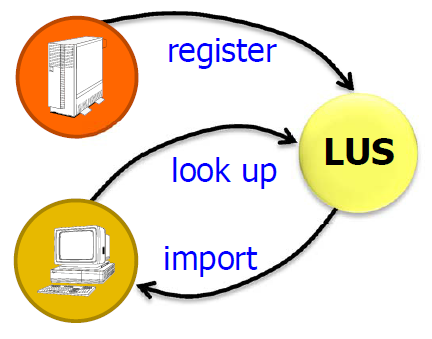
\includegraphics[scale=0.3]{./Bilder/Lookup-Service}
\end{figure}

\paragraph{Vorteile}
\begin{itemize}
\item mehrere Server für gleichen Server registrieren
\item Autorisierung etc. überprüfen
\item duroch Polling der Server Verfügbarkeit eines Services testen
\item verschiedene Versionen eines Dienstes verwalten
\end{itemize}
\paragraph{Probleme}
\begin{itemize}
\item lookup kostet Ausführungszeit
\item zentraler LUS ist potentieller Engpass
\end{itemize}

\subsection{Web Services, Middleware}
\textit{Übersprungen}

\subsection{REST}
\textit{Übersprungen}

\subsection{Jini}
\textit{Übersprungen}

\subsection{Broadcast/Multicast}
\begin{description}
\item[Broadcast]\hfill\\
Senden an die Gesamtheit aller Teilnehmer
\item[Multicast]\hfill\\
Senden an eine Untergruppe aller Teilnehmer (Broadcast bezogen auf Untergruppe)
\end{description}

\subsubsection{"Best Effort" Broadcast}
\begin{itemize}
\item Euphemistische Bezeichnung da keine extra Anstrengung (einfache Realisierung ohne ACK etc.)
\item Keinerlei Garantien: unbestimmt wie viele / welche Empfänger erreicht wurden, unbestimmte Empfangsreihenfolge
\item Im Erfolgsfall effizient
\item Geeignet für Verbreitung unkritischer Informationen
\end{itemize}

\subsubsection{"Reliable" Broadcast}
\begin{itemize}
\item Ziel: Unter gewissen Fehlermodellen "möglichst zuverlässigen" Broadcast-Dienst realisieren
\item Idee: ACK für jede Einzelnachricht
\begin{itemize}[topsep=-100ex]
\item viele ACKs $\rightarrow$ Belastung des Servers $\rightarrow$ schlechte Skalierbarkeit
\end{itemize}
\item Idee: NACKs (negative ACKs):
\begin{itemize}
\item Alle Broadcasts werden nummeriert $\rightarrow$ Lücke wird erkannt beim Empfänger
\item NACK bzgl. fehlender Nachricht wird gesendet
\item Fehlende Nachricht wird nachgeliefert
\end{itemize}
\end{itemize}

\subsubsection{Broadcast: Empfangsreihenfolge}
\begin{description}
\item[FIFO-Broadcast]\hfill\\
Alle Broadcasts ein und des selben Selbers an eine Gruppe kommen bei allen Mitgliedern in FIFO-Reihenfolge an
\item[Kausale Nachrichtenabhängigkeit]\hfill\\
Von links nach rechts verlaufender Pfad von $X$ nach $Y$ $\rightarrow$ $Y$ hängt kausal von $X$ ab
\item[Kausaler Broadcast]\hfill\\
$N$ hängt kausal von $M$ ab, Prozess $P$ empfängt $M$ und $N$ $\rightarrow$ $P$ muss $M$ vor $N$ empfangen
\item[Atomarer Broadcast]\hfill\\
Prozesse $P_i$ und $P_j$ empfangen beide $M$ und $N$. $P_i$ empfängt $M$ vor $N$ genau dann, wenn $P_j$ $M$ vor $N$ empfängt
\end{description}

\begin{figure}[h]
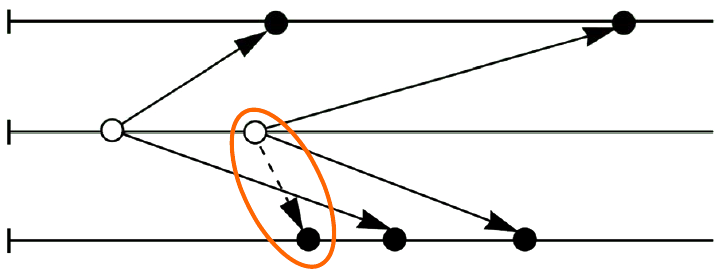
\includegraphics[height=2.5cm]{./Bilder/FIFO_Broadcast}
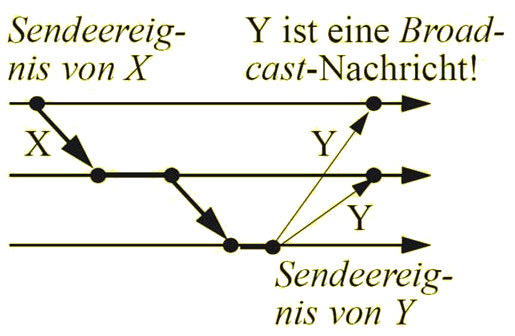
\includegraphics[height=2.5cm]{./Bilder/Kausaler_Broadcast}
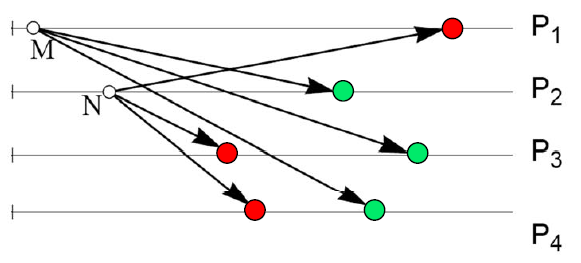
\includegraphics[height=2.5cm]{./Bilder/Atomarer_Broadcast}
\caption{FIFO, Kausal, Atomar}
\end{figure}

\paragraph{Eigenschaften:}
\begin{itemize}[topsep=-100ex]
\item Atomar $\nRightarrow$ kausal
\item Atomar $\nRightarrow$ FIFO
\item Atomar + FIFO $\nRightarrow$ kausal
\end{itemize}


\subsection{Logische Zeit}
\begin{description}
\item[Definition Kausalrelation $\prec$]\hfill\\
x $\prec$ y genau dann, wenn:
\begin{enumerate}[topsep=-100ex]
\item x und y auf dem gleichen Prozess stattfinden und x vor (links von) y kommt, oder
\item x ist ein Sendeereignis und y ein korrespondierendes Empfangsereignis, oder
\item $\exists$ z mit x $\prec$ z $\wedge$ z $\prec$ y
\end{enumerate}
\item[Definition C(e) (Zeitstempel)]\hfill\\
Wenn C(e) $<$ C(e') dann nennt man e früher als e'
\item[Uhrenbedingung]\hfill\\
e $\prec$ e' $\Rightarrow$ C(e) $<$ C(e') (Zeit ist kausaltreu)
\end{description}

\subsubsection{Lamport-Uhren}
\begin{itemize}
\item Bei jedem Ereignis tickt lokale Uhr (=Zähler) des Prozesses
\item Senden: aktuellen Uhrwert mitsenden (Zeitstempel der Nachricht)
\item Empfangen: Uhr = max(Uhr, Zeitstempel der Nachricht) (zuerst max(), anschliessend ticken)
\end{itemize}

\begin{description}
\item[Injektive Variante]\hfill\\
Lexikographische Ordnung (C(e),i), i ist Prozessnummer auf dem e stattfindet\\
(a,b) $<$ (a',b') $\Leftrightarrow$ a $<$ a' $\vee$ a = a' $\wedge$ b $<$ b'
\end{description}


\subsection{Wechselseitiger Ausschluss}
\subsubsection{Anforderungen}
\begin{description}
\item[Safety] Nothing bad will ever happen
\item[Liveness] Something good will eventually happen
\item[Fairness] Jeder kommt mal zum Zug
\end{description}

\subsubsection{Zentraler Manager}
\begin{itemize}
\item Manager ordnet Ressourcen exklusiv aber fair zu
\item Problem: Single point of failure
\end{itemize}

\subsubsection{Warteschlange}
\paragraph{Globale Warteschlange}
\begin{itemize}
\item Zentraler Manager-Prozess hält zeitlich geordnete FIFO Warteschlange von Requests
\item Problem: Single point of failure
\end{itemize}

\paragraph{Replizierte Warteschlange}
\begin{itemize}
\item Warteschlange bei jedem Prozess replizieren
\item Alle Prozesse sollen gleiche Sicht haben
\item Konsistenz wird mit Nachrichten und logischer Zeit erreicht
\item Voraussetzungen: FIFO-Kommunikationskanäle, eindeutige Zeitstempel, FIFO-Broadcast, Request werden geACKt
\end{itemize}

\subsubsection{Lamport Algorithmus}
\begin{enumerate}
\item Bewerbung um BM: Request mit Zeitstempel und Absender an alle senden und in eigene Queue einfügen
\item Empfang eines Requests: Request in eigene Queue einfügen, ACK versenden
\item Freigabe des BM: Aus eigener Queue entfernen und Release an alle senden
\item Emfpang eines Releases: Zugehörigen Request aus eigener Queue entfernen
\end{enumerate}
Ein Prozess darf BM nuten wenn:
\begin{enumerate}[label=\alph*.]
\item Eigener Request ist frühester in seiner Queue 
\item Von jedem anderen Prozess irgendeine spätere Nachricht bekommen
\end{enumerate}




\subsection{Sicherheit}
\textit{Übersprungen}

\end{document}
